\section{Supplementary Large-Scale Experiment}
\label{sec:large_scale}

To assess the scalability of exact solving paradigms beyond the $N=100$ boundary, an independent, supplementary experiment was conducted at $N=200$ (representing a board size of $200 \times 200$ with $40,000$ primary Boolean variables). A strict memory guard policy was introduced to prevent hardware exhaustion. Table~\ref{tab:n200_results} presents the solver outcomes based on $5$ isolated repetitions per method.

\begin{table}[h]
\centering
\caption{Large-scale experimental outcomes at $N=200$. Medians and means calculated over successful trials only.}
\label{tab:n200_results}
\resizebox{\linewidth}{!}{
\begin{tabular}{llrrrr}
\toprule
\textbf{Method} & \textbf{Status} & \textbf{Success/5} & \textbf{Median Time (s)} & \textbf{Peak RAM (MB)} \\
\midrule
SAT-Binary & SAT & 5 & 0.815 & 288.9 \\
SAT-Pairwise & NOT\_RUN\_RESOURCE\_POLICY & 0 & N/A & N/A \\
SAT-Sequential & TIMEOUT & 0 & N/A & 649.5 \\
SAT-Commander & SAT & 5 & 0.441 & 146.2 \\
SAT-Product & SAT & 5 & 0.627 & 165.1 \\
OR-Tools CP-SAT & SAT & 5 & 3.672 & 259.7 \\
IBM CP Optimizer & LICENSE\_ERROR & 0 & N/A & 87.1 \\
\bottomrule
\end{tabular}
}
\end{table}

The scaling results fundamentally underscore the intersection of mathematical formulation and hardware capacity. The SAT-Pairwise formulation, which creates $O(N^4)$ clauses, generated an estimated $13.2$ million clauses at $N=200$ requiring over $4$GB of continuous memory allocation, prompting the preflight resource guard to abort execution (\texttt{NOT\_RUN\_RESOURCE\_POLICY}). SAT-Sequential experienced universal timeouts, aligning with its exponentially degrading CDCL resolution time observed at lower values of $N$. Moreover, the IBM CP Optimizer encountered a \texttt{LICENSE\_ERROR} triggered by its Community Edition search space limit ($2^{1000}$ combinations), which is easily breached by the $N=200$ variables. 

\begin{figure}[h]
\centering
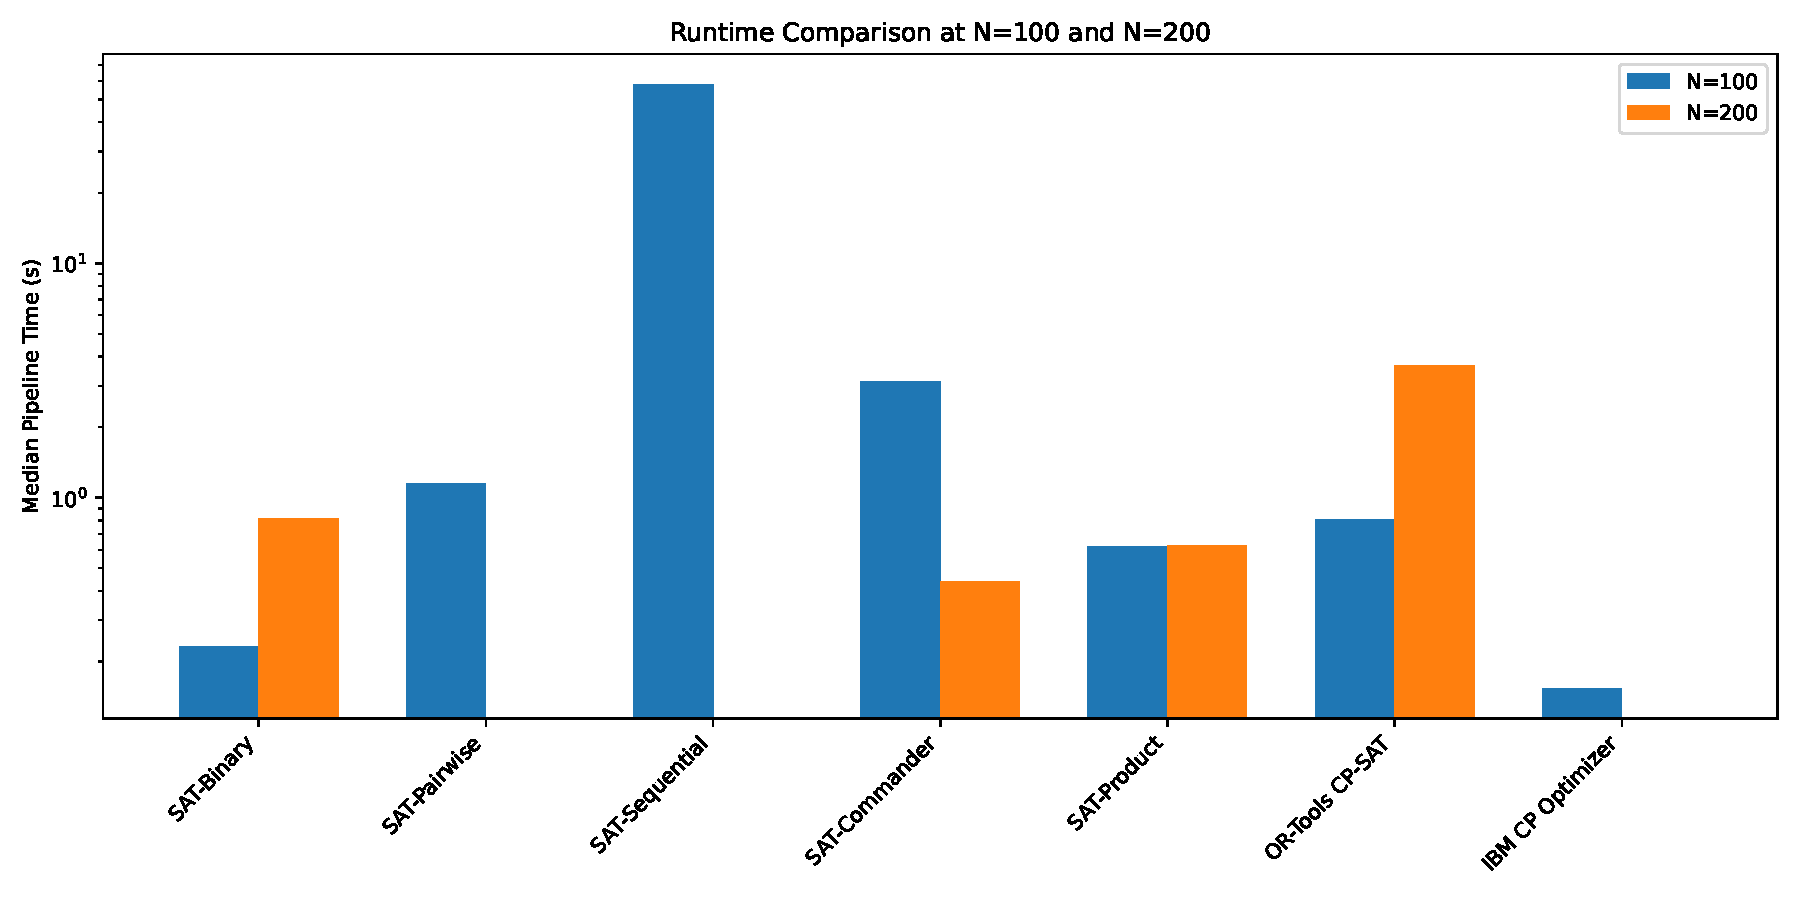
\includegraphics[width=0.8\textwidth]{../../results/figures/large_scale_n200/fig08_n100_vs_n200.pdf}
\caption{Median pipeline time comparison between $N=100$ and $N=200$ for successful methods.}
\label{fig:n100_vs_n200}
\end{figure}

As shown in Figure~\ref{fig:n100_vs_n200}, the methods that successfully scaled (SAT-Commander, SAT-Product, SAT-Binary, and OR-Tools CP-SAT) maintained manageable memory footprints due to their structural compactness. Interestingly, the SAT-Product encoding, which previously displayed non-monotonic failures and pathological timeouts at $N=44$ and $N=64$, effectively recovered at $N=200$ to achieve a median runtime of 0.627 seconds. Furthermore, SAT-Commander exhibited an inverted runtime scaling ratio (faster at $N=200$ than $N=100$), underscoring how specific variable partitioning strategies can favorably align with the default phase-saving heuristics of modern CDCL architectures on large symmetric grids.
